% Author: Izaak Neutelings (December 2022)
\documentclass[border=3pt,tikz]{standalone}
\usepackage{physics}
\usepackage{graphicx}
\usetikzlibrary{angles,quotes} % for pic (angle labels)
\tikzset{>=latex}

\colorlet{myred}{red!70!black}
\colorlet{myblue}{blue!80!black}
\colorlet{mygreen}{green!75!black}
\colorlet{pixelcol}{green!75!black}
\colorlet{trackcol}{red!75!black}
\tikzstyle{label}=[font=\bfseries,scale=1.3] %\sffamily]
\tikzstyle{mybox}=[line width=0.2,rounded corners=1pt] %,densely dashed]

\pgfdeclarelayer{back} % to draw on background
\pgfsetlayers{back,main} % set order
\def\mybox[#1]#2{
  \begin{pgfonlayer}{back} % draw on back
    \fill[mybox,#1!5] #2
  \end{pgfonlayer}
  \draw[mybox,#1] #2
}
\newcommand\p{\raisebox{.2ex}{+}}

\begin{document}

% ADD LABELS
\begin{tikzpicture}[x=1cm,y=1cm]
  
  % MAIN FIGURE
  \def\w{27.34cm} % width fine-tuned to match grid
  \node[inner sep=0,outer sep=0,above right] at (-0.0925*\w,-0.0345*\w) {
    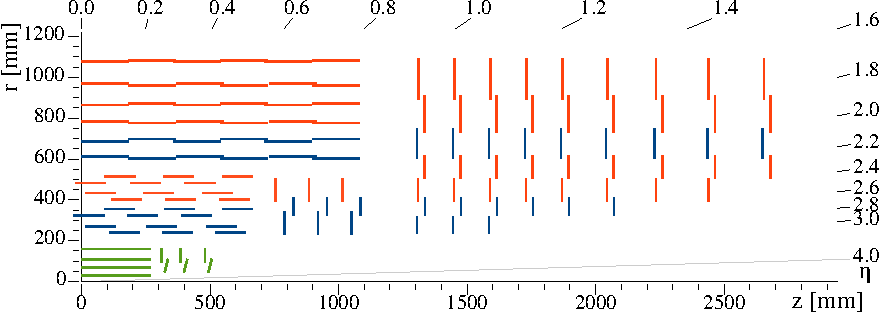
\includegraphics[width=\w]{CMS_tracker_Phase1.pdf}
  };
  
  %% HELP GRID
  %\draw[red,very thin,dashed] (0,0) grid[step=1cm] (20,8);
  %\draw[red,very thin] (0,0) grid[step=2cm] (20,8);
  %\fill[red!80!black] (0,0) circle(0.5mm);
  
  % PIXEL
  \mybox[mybox,pixelcol]{ (-0.1,-0.02) rectangle (2.25,1.15); }
  \mybox[mybox,pixelcol]{ (2.35,0.22) rectangle (4.2,1.12); }
  \node[label,pixelcol,left] at (-0.1,0.7) {BPIX};
  \node[label,pixelcol,right] at (4.2,0.45) {FPIX};
  
  % INNER
  \mybox[mybox,trackcol]{ (-0.3,1.35) rectangle (5.45,3.5); }
  \mybox[mybox,trackcol]{ (5.8,1.35) rectangle (8.95,3.35); }
  %\node[label,trackcol,left] at (-0.3,3.3) {TIB};
  \node[label,trackcol,below] at (5.2,1.35) {TIB};
  \node[label,trackcol,below] at (8.5,1.35) {TID\p};
  
  % OUTER
  \mybox[mybox,trackcol]{ (-0.1,3.65) rectangle (8.95,7.1); }
  \node[label,trackcol,above] at (3,7.1) {TOB};
  
  % ENDCAP
  \mybox[mybox,trackcol]{ (10.2,1.1) |- (21.8,7.1) --++ (0,-4.6) -- cycle; }
  \node[label,trackcol,above] at (15,7.1) {TEC\p};
  
\end{tikzpicture}

\end{document}
